\documentclass[12 pt, twoside] {article}
\usepackage[margin=1in]{geometry}
\usepackage[utf8]{inputenc}
\usepackage{listings}
\usepackage{color}
\usepackage{textcomp}
\usepackage{setspace}
\usepackage{verbatim}
\usepackage{graphicx}
\usepackage{footnote}
\usepackage{enumitem}
\makesavenoteenv{tabular}
\makesavenoteenv{table}

\setlist[itemize]{noitemsep, topsep=0pt}

\newcommand\la{\textlangle}
\newcommand\ra{\textrangle}

\setlength{\parindent}{0pt}

\definecolor{codegreen}{rgb}{0,0.6,0}
\definecolor{codegray}{rgb}{0.5,0.5,0.5}
\definecolor{codeblue}{rgb}{0,0,0.6}
\definecolor{backcolor}{rgb}{0.95,0.95,0.95}

\lstdefinestyle{mystyle}{
	backgroundcolor = \color{backcolor},
	commentstyle = \color{codeblue},
	keywordstyle = \color{codegreen},
	numberstyle = \color{codegray},
	stringstyle = \color{magenta},
	basicstyle = \footnotesize\ttfamily,
	breakatwhitespace = false,
	breaklines = true,
	captionpos = b,
	keepspaces = true,
	numbers = left,
	numbersep = 5pt,
	showspaces = false,
	showstringspaces = false,
	showtabs = false,
	tabsize = 4
}

\lstset{style = mystyle}

\begin{document}
{\catcode`?=\active
\def?!#1!{\footnote{#1}}

\section*{C++ Basics}
\subsection*{Structs and Class}

In vanilla C, structs are collections of variables, originally created for
custom typing. In C++, structs and classes are the same and have the same
function as any other object oriented language. The only difference between the
two is that in structs, variables and methods are by default public and in
classes they are by default private. This basically means that for the purpose
of competitive programming we almost always want to use structs.

The following is an example of a struct used to keep tract of a product on sale:
\begin{lstlisting}[language=c++]
// this is a declaration of a struct
// it follows the general pattern of
// struct <struct_name> {
//     <member_type_1> <member_name_1>;
//     <member_type_2> <member_name_2>;
//     . . . . . .
//     <method_type_1> <method_name_1>(<params>) {<implementation>};
// };
struct product {
    string name;
    double price;
    bool avaliable;

    // since structs and classes are the same, we can define constructors
    product(string a_name, double a_price) {
        name = a_name;
        price = a_price;
        avaliable = true;
    };

    // we can also define our own comparison operators, default behavior
    // is very glitchy so it is recommended if you want to sort an array
    // of this type to define your own comparison
    bool operator < (const product &B) const {
        return price < B.price;
    };
};

// to create an element of the type product you can use a constructor
product apple("apple", 6.5);
// or in c++11 you can initialize any struct with list initialization
// by default the order of arguments provided is the order of struct
// members in the definition, but you can also specify
// omitted values are given the default value of the type
product banana = {"banana", 3.33, true}; // <- for our purposes use this
product orange = {.price = 3.33, .name = "orange", .avaliable = true};
\end{lstlisting}
\subsection*{Lambda Expression}

Lambda expressions are inline anonymous functions especially helpful when using
certain functions in \texttt{algorithms} when doing special comparison. The
following example is an implementation of something similar to filter in cpp:
\begin{lstlisting}[language=c++]
#define T 5

void filterAbove(vector<int> &v) {
    // the syntax for a lambda expression is
    // [<capture group>](<argument list>) -> <ret type> { <code> }
    // the return type along with -> are often omitted for simple code
    // because the compiler can guess the return type.
    // the capture group is what the lambda function ``captures'' from the
    // surrounding namespace, for competitive programming purposes leave
    // it empty and just use #define statements up top.
    transform(v.begin(), v.end(), [](double d) { return d > T ? d : 0 });
}
\end{lstlisting}
\subsection*{Pointers}

Don't use them on purpose... Just know that \texttt{*p} dereferences a pointer
and \texttt{p+1} accesses the address at \texttt{p+} the size of the type of
pointer that \texttt{p} is.

\section*{C++ Containers}
\subsection*{vectors}

\begin{table}[h]
\centering
\begin{tabular}{|l|l|l|}
\hline
\multicolumn{3}{|c|}{\textbf{Constructors}}                                                                              \\ \hline
\texttt{vector\textless T\textgreater v;}             & Make an empty vector.                                   & O(1)             \\ \hline
\texttt{vector\textless T\textgreater v(n);}          & Make a vector with N elements.                          & O(n)             \\ \hline
\texttt{vector\textless T\textgreater v(n, value);}   & Make a vector with N elements, initialized to value.    & O(n)             \\ \hline
\texttt{vector\textless T\textgreater v(begin, end);} & Make a vector and copy the elements from begin to end.  & O(n)             \\ \hline
\multicolumn{3}{|c|}{\textbf{Accessors}}                                                                                 \\ \hline
\texttt{v{[}i{]};}                                   & Return (or set) the I'th element.                       & O(1)             \\ \hline
\texttt{v.at(i);}                                    & Return (or set) the I'th element, with bounds checking. & O(1)             \\ \hline
\texttt{v.size();}                                   & Return current number of elements.                      & O(1)             \\ \hline
\texttt{v.empty();}                                  & Return true if vector is empty.                         & O(1)             \\ \hline
\texttt{v.begin();}                                  & Return random access iterator to start.                 & O(1)             \\ \hline
\texttt{v.end();}                                    & Return random access iterator to end.                   & O(1)             \\ \hline
\texttt{v.front();}                                  & Return the first element.                               & O(1)             \\ \hline
\texttt{v.back();}                                   & Return the last element.                                & O(1)             \\ \hline
\texttt{v.capacity();}                               & Return maximum number of elements.                      & O(1)             \\ \hline
\multicolumn{3}{|c|}{\textbf{Modifiers}}                                                                                 \\ \hline
\texttt{v.push\_back(value);}                        & Add value to end.                                       & O(1)*  \\ \hline
\texttt{v.insert(iterator, value);}                  & Insert value at the position indexed by iterator.       & O(n)             \\ \hline
\texttt{v.pop\_back();}                              & Remove value from end.                                  & O(1)             \\ \hline
\texttt{v.erase(iterator);}                          & Erase value indexed by iterator.                        & O(n)             \\ \hline
\texttt{v.erase(begin, end);}                        & Erase the elements from begin to end.                   & O(n)             \\ \hline
\end{tabular}
\end{table}

\subsection*{lists}
\begin{table}[h]
\centering
\begin{tabular}{|l|l|l|}
\hline
\multicolumn{3}{|c|}{\textbf{Constructors}}                                                                 \\ \hline
\texttt{list\textless T\textgreater l;            } & Make an empty list.                                & O(1)       \\ \hline
\texttt{list\textless T\textgreater l(begin, end);} & Make a list and copy the values from begin to end. & O(n)       \\ \hline
\multicolumn{3}{|c|}{\textbf{Accessors}}                                                                    \\ \hline
\texttt{l.size(); }                                & Return current number of elements.                 & O(1)       \\ \hline
\texttt{l.empty();}                                & Return true if list is empty.                      & O(1)       \\ \hline
\texttt{l.begin();}                                & Return bidirectional iterator to start.            & O(1)       \\ \hline
\texttt{l.end();  }                                & Return bidirectional iterator to end.              & O(1)       \\ \hline
\texttt{l.front();}                                & Return the first element.                          & O(1)       \\ \hline
\texttt{l.back(); }                                & Return the last element.                           & O(1)       \\ \hline
\multicolumn{3}{|c|}{\textbf{Modifiers}}                                                                    \\ \hline
\texttt{l.push\_front(value);      }               & Add value to front.                                & O(1)       \\ \hline
\texttt{l.push\_back(value);       }               & Add value to end.                                  & O(1)       \\ \hline
\texttt{l.insert(iterator, value); }               & Insert value after position indexed by iterator.   & O(1)       \\ \hline
\texttt{l.pop\_front();            }               & Remove value from front.                           & O(1)       \\ \hline
\texttt{l.pop\_back();             }               & Remove value from end.                             & O(1)       \\ \hline
\texttt{l.erase(iterator);         }               & Erase value indexed by iterator.                   & O(1)       \\ \hline
\texttt{l.erase(begin, end);       }               & Erase the elements from begin to end.              & O(1)       \\ \hline
\texttt{l.remove(value);           }               & Remove all occurrences of value.                   & O(n)       \\ \hline
\texttt{l.remove\_if(test);        }               & Remove all element that satisfy test.              & O(n)       \\ \hline
\texttt{l.reverse();               }               & Reverse the list.                                  & O(n)       \\ \hline
\texttt{l.sort();                  }               & Sort the list.                                     & O(n log n) \\ \hline
\texttt{l.sort(comparison);        }               & Sort with comparison function.                     & O(n log n)  \\ \hline
\texttt{l.merge(l2);               }               & Merge sorted lists.                                & O(n)       \\ \hline
\end{tabular}
\end{table}
\subsection*{deques}
\begin{table}[h]
\centering
\begin{tabular}{|l|l|l|}
\hline
\multicolumn{3}{|c|}{\textbf{Constructors}}                                                                                      \\ \hline
\texttt{deque\textless T\textgreater d;}             & Make an empty deque.                                    & O(1)             \\ \hline
\texttt{deque\textless T\textgreater d(n);}          & Make a deque with N elements.                           & O(n)             \\ \hline
\texttt{deque\textless T\textgreater d(n, value);}   & Make a deque with N elements, initialized to value.     & O(n)             \\ \hline
\texttt{deque\textless T\textgreater d(begin, end);} & Make a deque and copy the values from begin to end.     & O(n)             \\ \hline
\multicolumn{3}{|c|}{\textbf{Accessors}}                                                                                         \\ \hline
\texttt{d{[}i{]}; }                                 & Return (or set) the I'th element.                       & O(1)             \\ \hline
\texttt{d.at(i);  }                                 & Return (or set) the I'th element, with bounds checking. & O(1)             \\ \hline
\end{tabular}
\end{table}
\newpage
\begin{table}
    \begin{tabular}{|l|l|l|}\hline
\texttt{d.size(); }                                 & Return current number of elements.                      & O(1)             \\ \hline
\texttt{d.empty();}                                 & Return true if deque is empty.                          & O(1)             \\ \hline
\texttt{d.begin();}                                 & Return random access iterator to start.                 & O(1)             \\ \hline
\texttt{d.end();  }                                 & Return random access iterator to end.                   & O(1)             \\ \hline
\texttt{d.front();}                                 & Return the first element.                               & O(1)             \\ \hline
\texttt{d.back(); }                                 & Return the last element.                                & O(1)             \\ \hline
\multicolumn{3}{|c|}{\textbf{Modifiers}}                                                                                         \\ \hline
\texttt{d.push\_front(value);      }                & Add value to front.                                     & O(1)* \\ \hline
\texttt{d.push\_back(value);       }                & Add value to end.                                       & O(1)* \\ \hline
\texttt{d.insert(iterator, value); }                & Insert value at the position indexed by iterator.       & O(n)             \\ \hline
\texttt{d.pop\_front();            }                & Remove value from front.                                & O(1)             \\ \hline
\texttt{d.pop\_back();             }                & Remove value from end.                                  & O(1)             \\ \hline
\texttt{d.erase(iterator);         }                & Erase value indexed by iterator.                        & O(n)             \\ \hline
\texttt{d.erase(begin, end);       }                & Erase the elements from begin to end.                   & O(n)             \\ \hline
\end{tabular}
\end{table}
\subsection*{stacks and queues}
In C++ STL, stacks and queues are \textit{container adaptors}, so they are
created from another container (one of the ones listed above, default to
vector).
\begin{table}[h]
    \begin{tabular}{|l|l|l|}\hline
        \multicolumn{3}{|c|}{\textbf{Constructors}}\\\hline
        \texttt{stack< container<T> > s;} & Make an empty stack. & O(1)\\\hline
        \texttt{queue< container<T> > q;} & Make an empty queue. & O(1)\\\hline
        \multicolumn{3}{|c|}{\textbf{Accessors}}\\\hline
        \texttt{s.top(); q.front(); q.back()} & Returns the top/front/back element. & O(1) \\\hline
        \texttt{s.size(); q.size();} & Returns current number of elements & O(1) \\\hline
        \texttt{s.empty(); q.empty();} & Returns true if empty & O(1) \\\hline
        \multicolumn{3}{|c|}{\textbf{Modifiers}}\\\hline
        \texttt{s.push(v); q.push(v)} & Push value to top/end & varies \\\hline
        \texttt{s.pop(); q.pop()} & Removes value from the top/front & O(1) \\\hline
    \end{tabular}
\end{table}

Note that the complexity of \texttt{push} varies depending on the underlying
container. But remember that it is always equal to the complexity of
\texttt{push\_back} for the underlying container.

\subsubsection*{priority queues}

This is also a \textit{container adaptor}. Except the element on top is
irrelevent of order of insertion. Instead the ``biggest'' element is on top.
Biggest is determined by the comparison predicate you give the priority queue constructor.
\begin{itemize}
    \item If that predicate is a ``less than'' type predicate, then biggest means largest.
    \item If it is a ``greater than'' type predicate, then biggest means smallest.
\end{itemize}

Again, the default container is a vector, the constructor is
\begin{verbatim}
priority_queue<T, container<T>, comparison<T> > q;
\end{verbatim}
and the complexity for push and pop are both O(n log n)
\subsection*{sets and multisets}
% Please add the following required packages to your document preamble:
% \usepackage{graphicx}
\begin{table}[h]
\centering
\begin{tabular}{|l|p{0.55\textwidth}|l|}
\hline
\multicolumn{3}{|c|}{\textbf{Constructors}}                                                                                                                                                                                                                       \\ \hline
\texttt{set<T, compare> s;}             & Make an empty set.
compare should be a binary predicate for ordering the set. It's optional and
will default to a function that uses \texttt{operator\textless}.
& O(1)       \\ \hline
\texttt{set<T, compare> s(begin, end);} &
Make a set and copy the values from begin to end.
& O(n log n) \\ \hline \multicolumn{3}{|c|}{\textbf{Accessors}}
\\ \hline
\texttt{s.find(key)  }                                          & Return an iterator pointing to an occurrence of key in s, or s.end() if key is not in s.                                                                                                    & O(log n)   \\ \hline
\texttt{s.lower\_bound(key)}                                    & Return an iterator pointing to the first occurrence of an item in s not less than key, or s.end() if no such item is found.                                                                 & O(log n)   \\ \hline
\texttt{s.upper\_bound(key)}                                    & Return an iterator pointing to the first occurrence of an item greater than key in s, or s.end() if no such item is found.                                                                  & O(log n)   \\ \hline
\texttt{s.equal\_range(key)}                                    & Returns pair\textlesslower\_bound(key), upper\_bound(key)\textgreater.                                                                                                                      & O(log n)   \\ \hline
\texttt{s.count(key) }                                          & Returns the number of items equal to key in s.                                                                                                                                              & O(log n)   \\ \hline
\texttt{s.size();    }                                          & Return current number of elements.                                                                                                                                                          & O(1)       \\ \hline
\texttt{s.empty();   }                                          & Return true if set is empty.                                                                                                                                                                & O(1)       \\ \hline
\texttt{s.begin()    }                                          & Return an iterator pointing to the first element.                                                                                                                                           & O(1)       \\ \hline
\texttt{s.end()      }                                          & Return an iterator pointing one past the last element.                                                                                                                                      & O(1)       \\ \hline
\multicolumn{3}{|c|}{\textbf{Modifiers}}                                                                                                                                                                                                                          \\ \hline
\texttt{s.insert(iterator, key)}                                & Inserts key into s. iterator is taken as a "hint" but key will go in the correct position no matter what. Returns an iterator pointing to where key went.                                   & O(log n)   \\ \hline
\texttt{s.insert(key)          }                                & Inserts key into s and returns a pair\textless iterator, bool\textgreater, where iterator is where key went and bool is true if key was actually inserted, i.e., was not already in the set. & O(log n)   \\ \hline
\end{tabular}%
\end{table}
\newpage
\subsection*{maps and multimaps}

\begin{table}[h]
\centering
\begin{tabular}{|p{0.3\textwidth}|p{0.6\textwidth}|l|}
\hline
\multicolumn{3}{|c|}{\textbf{Constructors}}                                                                                                                                                                                                                \\ \hline
\texttt{map<key\_type, value\_type, key\_compare> m;}             & Make an empty map. key\_compare should be a binary predicate for ordering the keys. It's optional and will default to a function that uses operator\textless. & O(1)       \\ \hline
\texttt{map<key\_type, value\_type, key\_compare> m(begin, end);} & Make a map and copy the values from begin to end.                                                                                                             & O(n log n) \\ \hline
\multicolumn{3}{|c|}{\textbf{Accessors}}                                                                                                                                                                                                                   \\ \hline
\texttt{m{[}key{]}           }                                                         & Return the value stored for key. This adds a default value if key not in map.                                                                                 & O(log n)   \\ \hline
\texttt{m.find(key)          }                                                         & Return an iterator pointing to a key-value pair, or m.end() if key is not in map.                                                                             & O(log n)   \\ \hline
\texttt{m.lower\_bound(key)  }                                                         & Return an iterator pointing to the first pair containing key, or m.end() if key is not in map.                                                                & O(log n)   \\ \hline
\texttt{m.upper\_bound(key)  }                                                         & Return an iterator pointing one past the last pair containing key, or m.end() if key is not in map.                                                           & O(log n)   \\ \hline
\texttt{m.equal\_range(key)  }                                                         & Return a pair containing the lower and upper bounds for key. This may be more efficient than calling those functions separately.                              & O(log n)   \\ \hline
\texttt{m.size();            }                                                         & Return current number of elements.                                                                                                                            & O(1)       \\ \hline
\texttt{m.empty();           }                                                         & Return true if map is empty.                                                                                                                                  & O(1)       \\ \hline
\texttt{m.begin()            }                                                         & Return an iterator pointing to the first pair.                                                                                                                & O(1)       \\ \hline
\texttt{m.end()              }                                                         & Return an iterator pointing one past the last pair.                                                                                                           & O(1)       \\ \hline
\multicolumn{3}{|c|}{\textbf{Modifiers}}                                                                                                                                                                                                                   \\ \hline
\texttt{m{[}key{]} = value;}                                                           & Store value under key in map.                                                                                                                                 & O(log n)   \\ \hline
\texttt{m.insert(pair)     }                                                           & Inserts the \textless key, value\textgreater pair into the map. Equivalent to the above operation.                                                             & O(log n)   \\ \hline
\end{tabular}
\end{table}
\newpage
\textbf{Choosing the Right Container}
\begin{figure}[h]
    \centering
    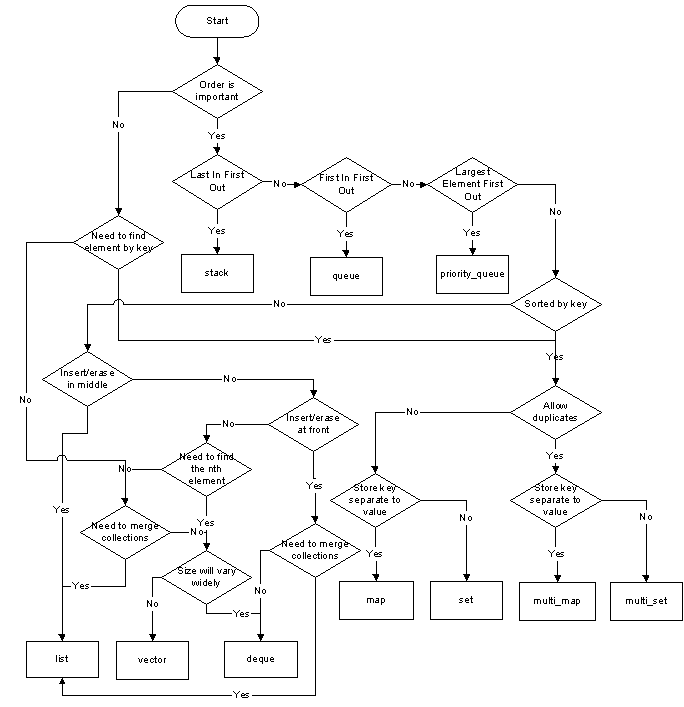
\includegraphics[width=0.9\textwidth]{containerchoice.png}
\end{figure}
\newpage
\subsection*{Algorithms}
\end{document}
